\begin{comment}
\subsection{Lifetime Contributions of Reciprocity-Activated Users}
%\placeholder{Include comparison of lifetime contributions for users whose first help was within seven days of receiving an answer vs.\ users whose first help was outside this window.}

\subsection{Alternative Observation Windows}
\label{sec:robustness_windows}
%\placeholder{Include results with 3-day, 5-day, and 14-day observation windows showing qualitative robustness of main findings.}

\subsection{Restricted Experience Analysis}
\label{sec:robustness_restricted}
%\placeholder{Include analysis restricted to users' first six activities, showing that reciprocity decline and response time moderation hold even within a narrow experience range.}

\subsection{Falsification Test}
\label{sec:falsification}
%\placeholder{Include results of the gap-period falsification test showing no significant effect during the waiting period.}

\subsection{Full Regression Tables}
\label{sec:full_tables}
%\placeholder{Include complete regression output for all models across all tenure buckets, including all covariates, standard errors, and model diagnostics.}
\end{comment}

\section{Matching Diagnostics}
\label{sec:balance_plot}
Figure \ref{fig:common_support} shows that there is sufficient common support between the treatment and the control group. The propensity score distribution between the original treated and control groups is similar. The distribution of the matched control is nearly identical to the treated group. 

\begin{figure}[!htbp]
    \centering
    \missingfigure{common\_support.pdf}
    \caption{Relationship between user experience and strength of status pursuit}
    \label{fig:common_support}
\end{figure}

Figure \ref{fig:love_plot} displays the standardized mean differences (SMD) between the matching variables before and after matching. While there are noticeable differences before the matching, all SMDs are very close to zero after the matching. 

\begin{figure}[!htbp]
    \centering
    \missingfigure{love\_plot.pdf}
    \caption{Visualization of balance in the unmatched and matched dataset}
    \label{fig:love_plot}
\end{figure}

\section{Help Rate Over the Observation Window by Tenure}
\label{sec:help_rate_by_tenure}

\begin{figure}[!htbp]
\centering
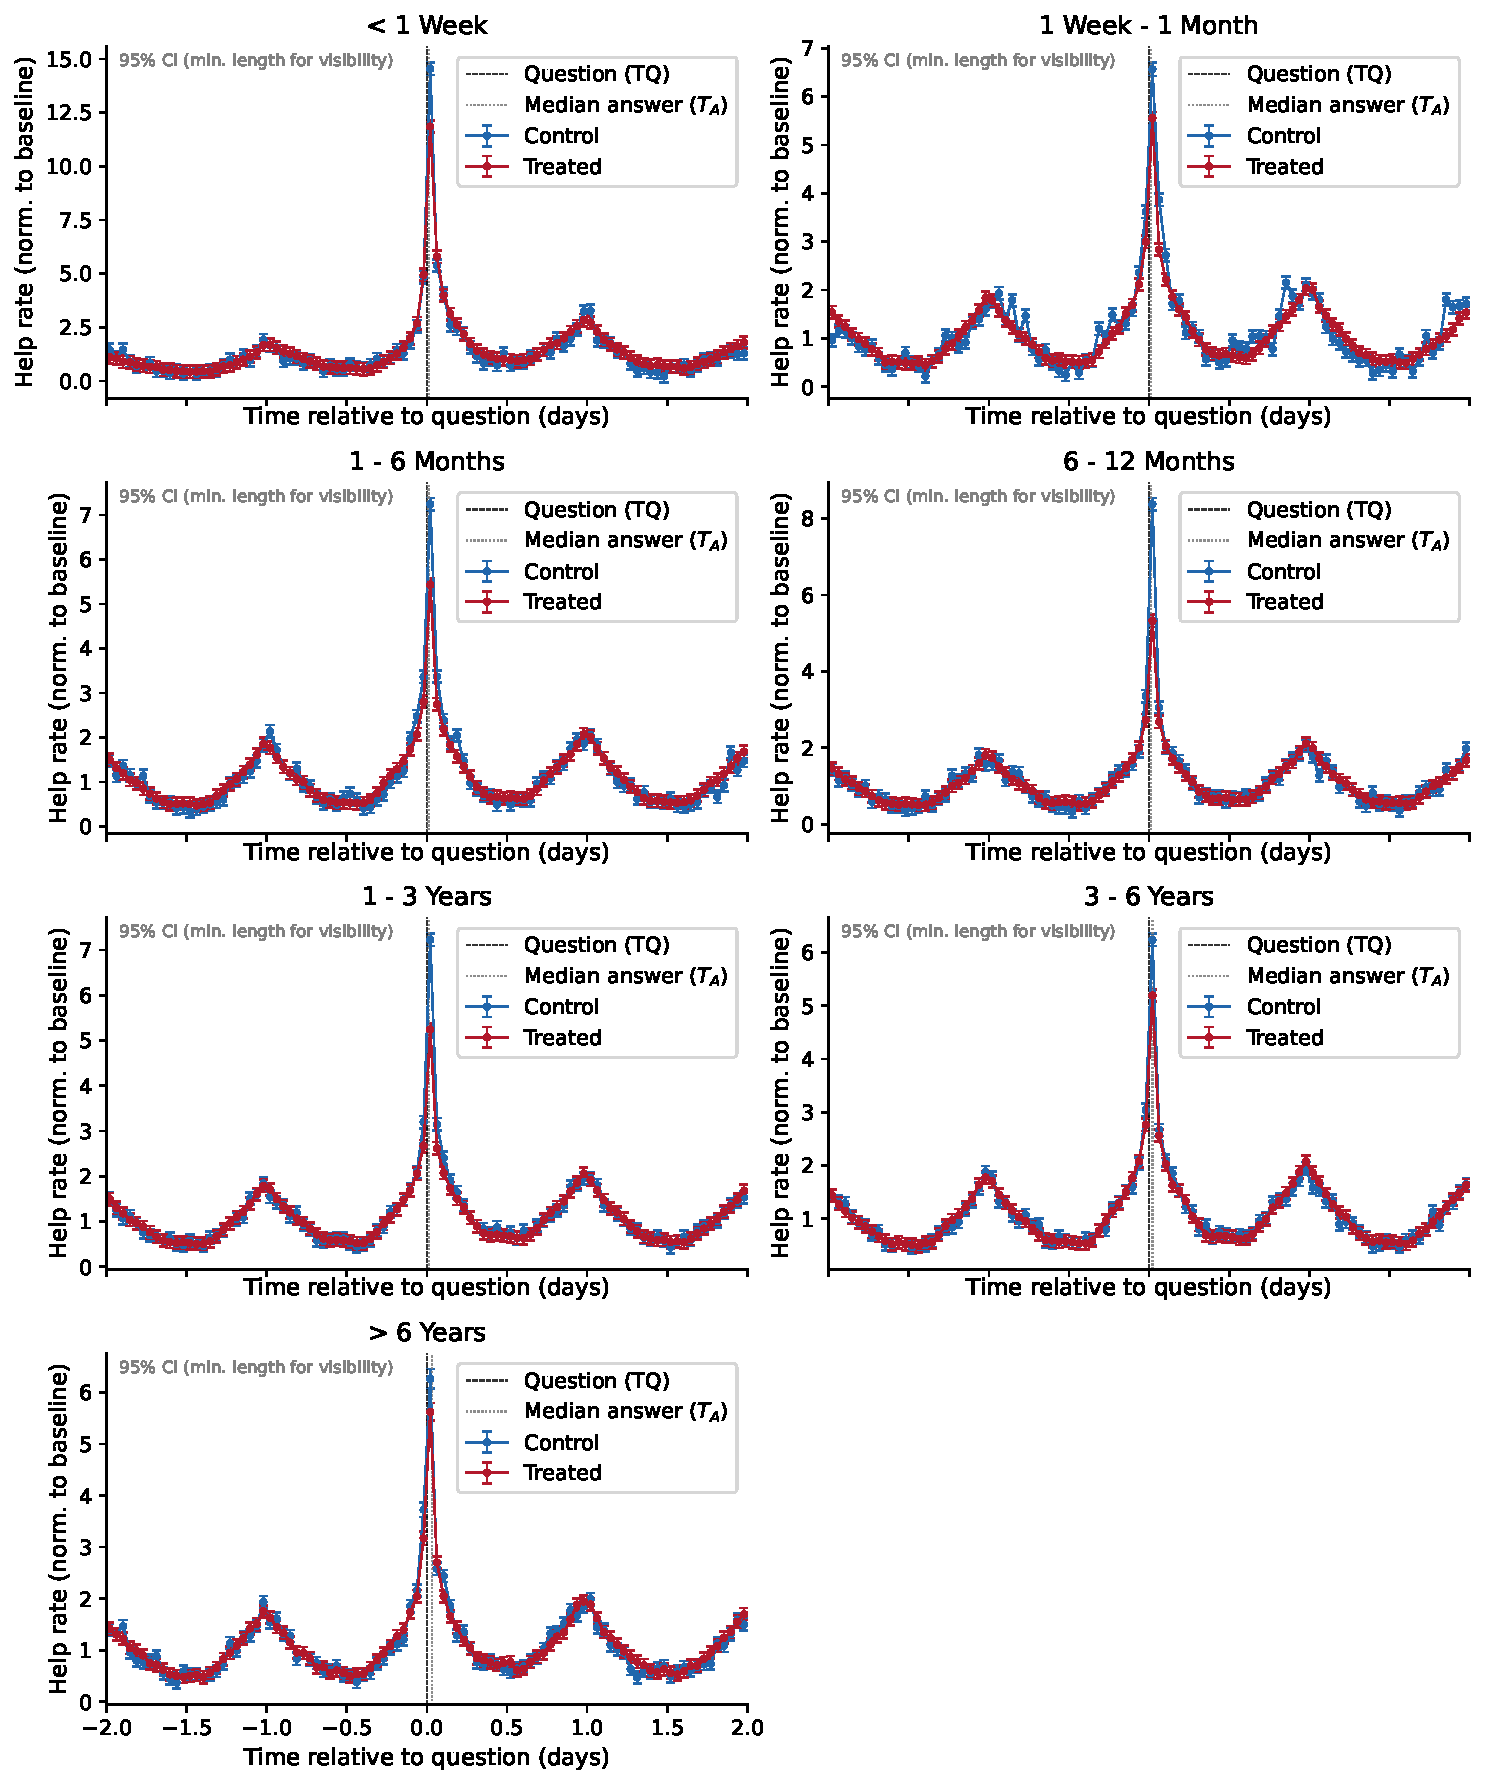
\includegraphics[width=\textwidth]{../analysis/output_figures/help_rate_by_tenure.pdf}
\caption{Help Rate Over the Observation Window, by Tenure Bucket. Each panel plots the normalized help rate (relative to each group's pre-question baseline) for treated users (red) and matched control users (blue) over the $\pm$2-day window around the question-posting time ($T_Q$, dashed vertical line). The dotted vertical line marks the median answer arrival time ($T_A$). Error bars indicate 95\% confidence intervals. The post-question lift in treated users' help rate is visible across all tenure buckets and is most pronounced among newcomers (tenure $<$ 1 week), consistent with the pattern reported in Table~\ref{tab:main_results} and Figure~\ref{fig:strength_rec}.}
\label{fig:help_rate_by_tenure}
\end{figure}

\section{Analysis of Life-Time Contributions \label{sec:lt-contributions}}
What remains unclear is whether users who become contributors through generalized reciprocity continue to contribute consistently and become valuable community members. To explore this, I compare the contributions of reciprocity-activated users with those of all contributors selected for Study 1. Specifically, I examine the number of times users from each group provided and received help up to July 14, 2024. The results are presented in Table \ref{tab:quartile_statistics}. Across all quartiles and at the median, reciprocity-activated users ask and provide more help than their counterparts.
For example, at the median, reciprocity-activated users provide eight answers and ask 13 questions, compared to six answers and 11 questions among all contributors. Similarly, the 75th percentile of reciprocity-activated users provides 23 answers and asks 29 questions, compared to 19 answers and 22 questions for all contributors.
These findings suggest that users who begin contributing after receiving help become equally, if not more, engaged in the community's helping dynamics compared to all contributors. Furthermore, this analysis demonstrates that once users start contributing, the act of giving and receiving help becomes (at least temporarily) decoupled.

\begin{table}[H]
\caption{Statistics on Contributions by User Sample}
\label{tab:quartile_statistics}
\centering
\begin{tabular}{lcccccc}
\toprule
 & \multicolumn{3}{c}{Answers Provided} & \multicolumn{3}{c}{Questions Asked} \\
\cmidrule(lr){2-4} \cmidrule(lr){5-7}
 & $Q_1$ & Med & $Q_3$ & $Q_1$ & Med & $Q_3$ \\
\midrule
Reciprocity-activated (\(N = 30,160\)) & 3.0 & 8.0 & 23.0 & 7.0 & 13.0 & 29.0 \\
All Contributors (\(N = 287,959\)) & 2.0 & 6.0 & 19.0 & 6.0 & 11.0 & 22.0 \\
\bottomrule
\end{tabular}
\end{table}

\iffalse
\begin{table}[caption={Linear Regression Results on Lifetime Contributions}, label={tab:quartile_statistics}]
\centering
\begin{tabular}{@{\extracolsep{1pt}}lcc} \toprule
& \multicolumn{2}{c}{Dependent Variable} \\ \cmidrule(lr){2-3}
& logNumberAnswers & logNumberComments \\
\midrule
activatedUser(1) & 0.081$^{***}$ & 0.187$^{***}$ \\ 
 & (0.007) & (0.010) \\ \rule{0pt}{4ex}%
 
numberQuestions & 0.007$^{***}$ & 0.008$^{***}$ \\ 
 & (0.000) & (0.001) \\ \rule{0pt}{4ex}%

Constant & 3.413$^{***}$ & 2.925$^{***}$ \\
 & (0.016) & (0.023) \\ \rule{0pt}{4ex}%
Year controls & YES & YES \\
\midrule
Observations & 287,959 & 287,959 \\
F-statistic & 3168$^{***}$ & 2498$^{***}$ \\ 
\bottomrule
\end{tabular}
\caption*{\raggedright \textit{Notes.} Significance levels: $^{*}$ \textit{p} < .05; $^{**}$\textit{p} < .01; $^{***}$\textit{p} < .001. Standard errors are reported in parentheses.}
\end{table}
\fi

\begin{comment}
\section{Robustness Checks \label{sec:robustness}}
To assess the robustness and consistency of my findings, I conducted a series of robustness checks that varied the observation length, the construction of the dependent variable \textit{numHelped}, or model specification.

I assessed the robustness of my findings by varying the observation length. While the reciprocity model used a seven-day observation length per period, I created two equivalent models with ten and three days of observation length. That is, I observe the helping behavior of the user three and ten days before and after receiving help, respectively. The results of these additional models (see Table \ref{tab:rec_models10d} and \ref{tab:rec_models3d}) are consistent with the above results and qualitatively equivalent, indicating that the findings are not sensitive to the specific observation length used.
\end{comment}
